% fig_mc_ci_summary.tex
% TR-26: CI summary bar chart for all three Monte Carlo groups
% Bars: observed rate (TPR for A,B / security rate for C)
% Whiskers: 95% Wilson CI
% Horizontal lines: performance targets (≥0.990 for TPR, ≥0.995 for security)
%
% Results from run_ibr_monte_carlo.py:
%   Group A (3PH TPR):    1.0000, CI [0.9992, 1.0000]
%   Group B (SLG TPR):    1.0000, CI [0.9992, 1.0000]
%   Group C (security):   1.0000, CI [0.9992, 1.0000]
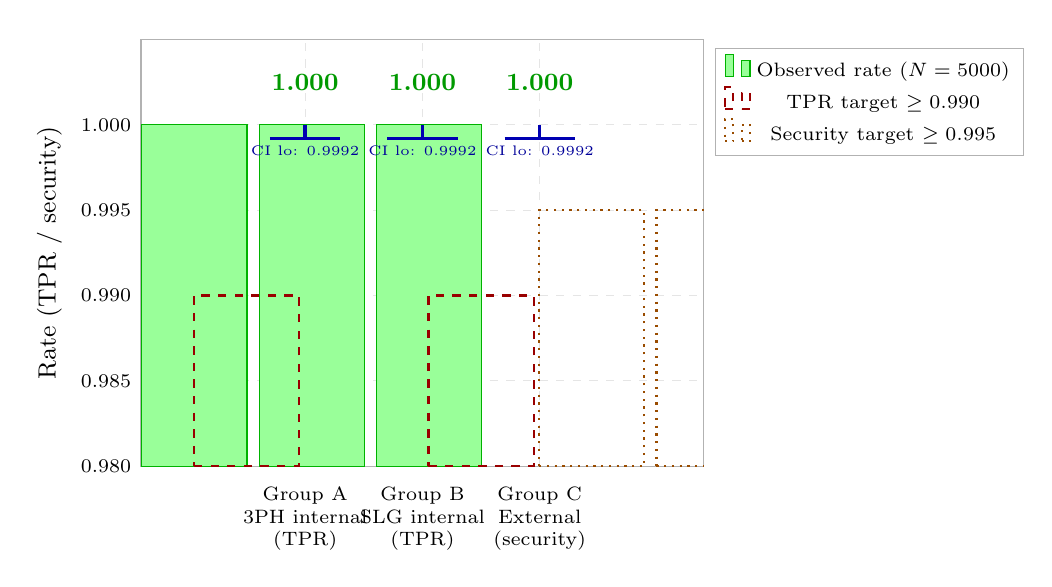
\begin{tikzpicture}
\begin{axis}[
  name        = ciax,
  ybar,
  bar width   = 38pt,
  width       = 0.72\textwidth,
  height      = 7.0cm,
  ylabel      = {Rate (TPR / security)},
  ylabel style= {font=\small},
  ymin=0.98, ymax=1.005,
  ytick       = {0.98, 0.985, 0.990, 0.995, 1.000},
  yticklabels = {0.980, 0.985, 0.990, 0.995, 1.000},
  yticklabel style={font=\scriptsize},
  xtick       = {1, 2, 3},
  xticklabels = {Group A\\3PH internal\\(TPR),
                 Group B\\SLG internal\\(TPR),
                 Group C\\External\\(security)},
  xticklabel style={font=\scriptsize, align=center},
  enlarge x limits=0.30,
  legend style={at={(1.02,0.98)}, anchor=north west,
                font=\scriptsize, draw=gray!60},
  grid       = major,
  grid style = {gray!20, dashed},
  tick style = {draw=none},
  axis line style={gray!60},
]

% Observed rates: all 1.000
\addplot[fill=green!40, draw=green!70!black]
  coordinates { (1, 1.000) (2, 1.000) (3, 1.000) };
\addlegendentry{Observed rate ($N=5000$)}

% Performance target lines
\addplot[red!60!black, thick, dashed, mark=none, domain=0.5:2.5, samples=2]
  ({x}, {0.990});
\addlegendentry{TPR target $\geq 0.990$}

\addplot[orange!60!black, thick, dotted, mark=none, domain=2.5:3.5, samples=2]
  ({x}, {0.995});
\addlegendentry{Security target $\geq 0.995$}

% CI whiskers — explicit per group
\draw[blue!70!black, very thick] (axis cs:1,1.000)--(axis cs:1,0.9992);
\draw[blue!70!black, thick]      (axis cs:0.7,0.9992)--(axis cs:1.3,0.9992);
\draw[blue!70!black, very thick] (axis cs:2,1.000)--(axis cs:2,0.9992);
\draw[blue!70!black, thick]      (axis cs:1.7,0.9992)--(axis cs:2.3,0.9992);
\draw[blue!70!black, very thick] (axis cs:3,1.000)--(axis cs:3,0.9992);
\draw[blue!70!black, thick]      (axis cs:2.7,0.9992)--(axis cs:3.3,0.9992);

% Rate labels
\node[font=\small\bfseries, green!60!black] at (axis cs:1, 1.0025) {1.000};
\node[font=\small\bfseries, green!60!black] at (axis cs:2, 1.0025) {1.000};
\node[font=\small\bfseries, green!60!black] at (axis cs:3, 1.0025) {1.000};

% CI lower bound label
\node[font=\tiny, blue!60!black] at (axis cs:1, 0.9985) {CI lo: 0.9992};
\node[font=\tiny, blue!60!black] at (axis cs:2, 0.9985) {CI lo: 0.9992};
\node[font=\tiny, blue!60!black] at (axis cs:3, 0.9985) {CI lo: 0.9992};

\end{axis}
\end{tikzpicture}
